\tikzset{every picture/.style={line width=0.75pt}} %set default line width to 0.75pt        

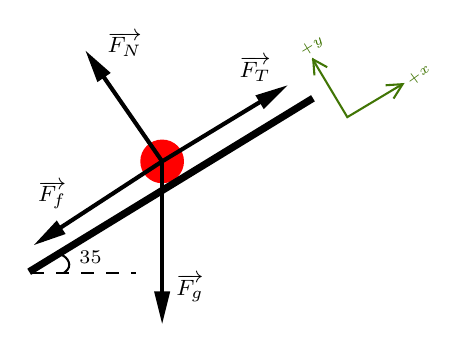
\begin{tikzpicture}[x=0.75pt,y=0.75pt,yscale=-1,xscale=1]
	%uncomment if require: \path (0,300); %set diagram left start at 0, and has height of 300

	%Shape: Ellipse [id:dp4017134135670819] 
	\draw  [color={rgb, 255:red, 255; green, 0; blue, 0 }  ,draw opacity=1 ][fill={rgb, 255:red, 255; green, 0; blue, 0 }  ,fill opacity=1 ] (111.34,112.66) .. controls (111.34,107.12) and (115.83,102.64) .. (121.37,102.64) .. controls (126.9,102.64) and (131.39,107.12) .. (131.39,112.66) .. controls (131.39,118.2) and (126.9,122.69) .. (121.37,122.69) .. controls (115.83,122.69) and (111.34,118.2) .. (111.34,112.66) -- cycle ;
	%Straight Lines [id:da11049691654941651] 
	\draw [line width=1.5]    (121.37,112.66) -- (86.79,62.71) ;
	\draw [shift={(84.51,59.43)}, rotate = 55.3] [fill={rgb, 255:red, 0; green, 0; blue, 0 }  ][line width=0.08]  [draw opacity=0] (15.6,-3.9) -- (0,0) -- (15.6,3.9) -- cycle    ;
	%Straight Lines [id:da9494684383086442] 
	\draw [line width=1.5]    (121.37,112.66) -- (121.37,186.86) ;
	\draw [shift={(121.37,190.86)}, rotate = 270] [fill={rgb, 255:red, 0; green, 0; blue, 0 }  ][line width=0.08]  [draw opacity=0] (15.6,-3.9) -- (0,0) -- (15.6,3.9) -- cycle    ;
	%Shape: Right Angle [id:dp18042975486392487] 
	\draw  [color={rgb, 255:red, 65; green, 117; blue, 5 }  ,draw opacity=1 ] (193.86,63.38) -- (210.59,91.34) -- (237.26,75.37) ;
	\draw  [color={rgb, 255:red, 65; green, 117; blue, 5 }  ,draw opacity=1 ] (229.05,75.99) -- (237.23,75.45) -- (232.86,82.39) ;
	\draw  [color={rgb, 255:red, 65; green, 117; blue, 5 }  ,draw opacity=1 ] (194.75,71.23) -- (194.15,63.58) -- (200.91,67.29) ;

	%Shape: Rectangle [id:dp3435108917878682] 
	\draw  [fill={rgb, 255:red, 0; green, 0; blue, 0 }  ,fill opacity=1 ] (58.37,166.64) -- (194.25,83.57) -- (192.96,81.45) -- (57.08,164.53) -- cycle ;
	%Straight Lines [id:da04201278790866225] 
	\draw [line width=1.5]    (121.37,112.66) -- (178.24,78.16) ;
	\draw [shift={(181.66,76.09)}, rotate = 148.76] [fill={rgb, 255:red, 0; green, 0; blue, 0 }  ][line width=0.08]  [draw opacity=0] (15.6,-3.9) -- (0,0) -- (15.6,3.9) -- cycle    ;
	%Straight Lines [id:da3784033887963598] 
	\draw [line width=1.5]    (121.37,112.66) -- (63.01,150.72) ;
	\draw [shift={(59.66,152.91)}, rotate = 326.89] [fill={rgb, 255:red, 0; green, 0; blue, 0 }  ][line width=0.08]  [draw opacity=0] (15.6,-3.9) -- (0,0) -- (15.6,3.9) -- cycle    ;
	%Curve Lines [id:da8374647738641394] 
	\draw    (74.27,166.2) .. controls (78.86,163.07) and (75.76,158.84) .. (72.93,157.71) ;
	%Straight Lines [id:da35140741666861075] 
	\draw  [dash pattern={on 4.5pt off 4.5pt}]  (58.37,166.64) -- (108.8,166.64) ;

	% Text Node
	\draw (93.59,48.74) node [anchor=north west][inner sep=0.75pt]  [font=\footnotesize] [align=left] {$\displaystyle \overrightarrow{F_{N}}$};
	% Text Node
	\draw (126.77,165.7) node [anchor=north west][inner sep=0.75pt]  [font=\footnotesize] [align=left] {$\displaystyle \overrightarrow{F_{g}}$};
	% Text Node
	\draw (236.41,72) node [anchor=north west][inner sep=0.75pt]  [font=\tiny,color={rgb, 255:red, 65; green, 117; blue, 5 }  ,opacity=1 ,rotate=-323.81] [align=left] {$\displaystyle +x$};
	% Text Node
	\draw (184.88,57.25) node [anchor=north west][inner sep=0.75pt]  [font=\tiny,color={rgb, 255:red, 65; green, 117; blue, 5 }  ,opacity=1 ,rotate=-328.27] [align=left] {$\displaystyle +y$};
	% Text Node
	\draw (157.19,60.68) node [anchor=north west][inner sep=0.75pt]  [font=\footnotesize] [align=left] {$\displaystyle \overrightarrow{F_{T}}$};
	% Text Node
	\draw (60.09,120.55) node [anchor=north west][inner sep=0.75pt]  [font=\footnotesize] [align=left] {$\displaystyle \overrightarrow{F_{f}}$};
	% Text Node
	\draw (80.04,154.12) node [anchor=north west][inner sep=0.75pt]  [font=\scriptsize] [align=left] {$\displaystyle 35\degree $};


\end{tikzpicture}